\question 假定某页式管理系统中,主存为128KB,分成32块,块号为0,1,2,3,,31;某作业有5块,其页号为0,1,2,3,4,被分别装入主存的3,8,4,6,9块中。有一逻辑地址为{[}3,70{]}。试求出相应的物理地址(其中方括号中的第一个元素为页号,第二个元素为页内地址,按十进制计算)(
~)
\par\twoch{14646}{\textcolor{red}{24646}}{24576}{34576}
\begin{solution}块大小为128KB/32=4KB,因为块与页面大小相等,所以每页为4KB。第3页被装入到主存第6块中,故逻辑地址{[}3,70{]}对应的物理地址为4K×6+70=24576+70=24646。
其地址变换过程如图3-23所示。
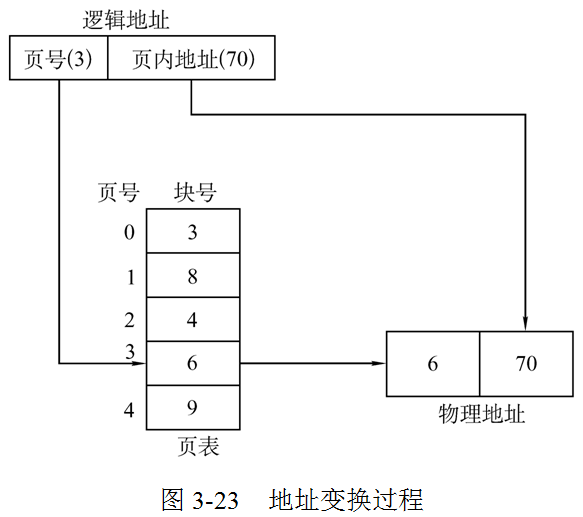
\includegraphics[width=3.33333in,height=2.94792in]{computerassets/65E8216F2268DF223B4B882D04D1F7BE.png}
\end{solution}
\question (南京理工大学,2002年)动态重定位是在作业的( )中进行的
\par\twoch{编译过程}{装入过程}{链接过程}{\textcolor{red}{执行过程}}
\begin{solution}(1)静态重定位在程序装入内存的过程中完成,是指在程序开始运行前,程序中的各个地址有关的项均已完成重定位。地址变换通常是在装入时一次完成的,以后不再改变,故称为静态重定位。
(2)动态重定位不是在程序装入内存时完成的,而是CPU每次访问内存时由动态地址变换机构(硬件)自动把相对地址转换为绝对地址。动态重定位需要软件和硬件相互配合完成。
\end{solution}
\question 下列存储管理方案中,可以采用静态重定位的是
\par\twoch{\textcolor{red}{固定分区管理方案}}{可变分区管理方案}{页式管理方案}{段式管理方案}
\begin{solution}在固定分区方式中,作业分区情况一旦确定便不会改变,故可以采用静态重定位。其余三种管理方案均可能在运行过程中改变作业分区情况,故不可以采用静态重定位。
\end{solution}
\question (武汉理工大学,2005年)下面的存储管理方案中,(
)方式可以采用静态重定位
\par\twoch{\textcolor{red}{固定分区}}{可变分区}{页式}{段式}
\begin{solution}静态重定位在程序装入内存的过程中完成,是指在程序开始运行前,程序中的各个地址有关的项均已完成重定位。地址变换通常是在装入时一次完成的,以后不再改变。
只有在固定分区方式中,作业分区情况一旦确定便不会改变,故可以采用静态重定位。其余3种管理方案均可能在运行过程中改变作业分区情况,故不可以采用静态重定位。
\end{solution}
\question 以下叙述错误的是
\par\twoch{\textcolor{red}{覆盖对程序员是透明的}}{交换对程序员是透明的}{在分页系统环境下,分页对程序员是透明的}{联想寄存器的地址变换对操作系统是透明的}
\begin{solution}覆盖对程序员是不透明的。为了节省内存,提高覆盖的效果,用户在编制程序时就要安排好程序的覆盖结构,覆盖的目的是希望运行更大的程序。
同为节省内存,覆盖技术用于一个作业的内部,交换技术则用于不同的作业。交换对程序员是透明的,交换的目的是希望能够运行更多的程序。
因此A错误,B正确。
C正确,分页的实现是由操作系统自动实现的,因此分页对程序员是透明的。
D正确,联想寄存器的地址变换是由硬件实施的,不需要通过操作系统软件(指令)实施。但在实施快表的淘汰算法时,要通过操作系统实施。
\end{solution}
\question 在运行过程中,许多系统允许程序分配更多的内存给它的地址空间。在程序堆中的数据分配是这种分配方式的一个实例。下列关于不同内存分配方式的说法错误的是
\par\fourch{连续内存分配方式下,当没有足够的空间给程序去扩大它已分配的内存空间时,将要求重新分配整个程序}{纯段式分配方式下,当没有足够的空间给段去扩大它的已分配内存空间时,将要求重新分配整个段}{\textcolor{red}{纯页式分配方式下,当需要扩大它的已分配内存空间时,将要求重新分配全部页}}{在段页式分配方式下,当需要扩大它的已分配内存空间时,系统不需要重新分配全部页}
\begin{solution}其实只要知道每种分配方式最小的内存单位(需要连续地址空间的最小块)是什么,答案就容易得出来了。连续内存分配方式下,最小的内存单位就是整个程序。当没有足够的空间去扩大已分配内存时,就需要重新分配整个程序。纯段式分配方式下,最小的内存单位就是段,当没有足够的空间去扩大已分配给段的内存时,就需要重新分配整个段。故A选项和B选项都是正确的。
纯页式分配方式下,它的内存单位(页)大小是不可变的,故不可能会有重新分配全部页的情况。C选项中提到的情况,只需要添加页表项即可,即增加新分配的页给程序的地址空间,故C选项错误。
段页式管理方式对于内存空间的分配也都是以页为单位的,所以不需要重新分配全部页,只要对每个段对应的页表添加页表项即可,故D选项正确。
\end{solution}
\question 假设页的大小为4KB,页表的每个表项占用4B。对于一个64位地址空间系统,采用多级页表机制,至少需要(
~)级页表(本题默认字长为1B)
\par\twoch{3}{4}{5}{\textcolor{red}{6}}
\begin{solution}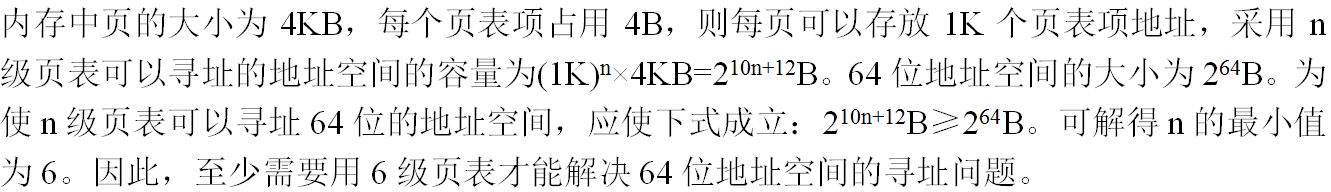
\includegraphics[width=3.46875in,height=0.50000in]{computerassets/243B0B774FFA6638E6FAB305AD26DD03.png}

4KB/1B=4k=2∧12,故页内地址为12位,总共64位,页地址为64-12=52位,每页可以存放4KB/4B=1k=2∧10个页表项,故一级页表可以索引2∧10个页,要索引2∧52个页,总共需要2∧52/2∧10=6(向上取整)级页表
\end{solution}
\question 在存储管理方案中,可用上、下限地址寄存器存储保护的是
\par\twoch{页式管理}{段式管理}{\textcolor{red}{固定分区管理}}{段页式管理}
\begin{solution}固定分区管理可采用静态重定位的方式装入作业。装入程序把作业中的逻辑地址转换为绝对地址,并检查绝对地址是否在指定(装入)的分区内,如果是,就装入这个作业;否则就不能装入。如果装入主存分区的作业占用处理器时(注意,是运行时),进程调度程序(不是装入程序了)必须把作业所在分区的上下限地址存入``下限寄存器''和``上限寄存器''中,这样可以在指令执行中判断其所用到的绝对地址是否越界,达到存储保护的目的。
其他选项的管理方式对于存储保护都是通过其他寄存器(或方式)来进行内存保护的。考生可自己总结。
\end{solution}
\question 在动态分区式内存管理中,首次适应算法的空闲区是
\par\twoch{\textcolor{red}{按地址递增顺序连在一起}}{始端指针表指向最大空闲区}{按大小递增顺序连在一起}{寻找从最大空闲区开始}
\begin{solution}以空闲分区链为例来说明采用首次适应算法(FF)时的分配情况。FF算法要求空闲分区链以地址递增的次序链接。在分配内存时,从链首开始顺序查找,直至找到一个大小能满足要求的空闲分区为止;然后再按照作业的大小,从该分区中划出一块内存空间分配给请求者,余下的空闲分区仍留在空闲链中。若从链首直至链尾都不能找到一个能满足要求的分区,则此次内存分配失败,返回。
\end{solution}
\question 在页式存储管理中选择页面的大小,需要考虑下列哪些因素( )。
Ⅰ.页表的大小 Ⅱ.内部碎片引起的内存浪费 Ⅲ.磁盘访问时间
\par\twoch{Ⅰ和Ⅲ}{\textcolor{red}{Ⅰ和Ⅱ}}{Ⅰ、Ⅱ和Ⅲ}{Ⅱ和Ⅲ}
\begin{solution}选择页面大小是一个需要权衡的问题。 较大页面的优点如下:
(1)页表的大小与页面的大小成反比,较大的页面可以节省实现地址映射所需的存储空间及其他资源。
(2)较大的页面可使虚拟存储器的实现更加简单。
(3)在主存和辅存之间传送较大页面比传送小页面更加有效。
(4)联想存储器(也称快表)的项数有限,对于同样项数的快表,较大页面意味着可高效实现更多存储空间的地址变换,从而减少快表失效的次数。
较小页面的优点如下: (1)节省存储空间,即减少内零头(内碎片)。
(2)节省进程的启动时间,许多进程都比较小,所以采用小页面可以加快进程的调用。
\end{solution}
\question 采用分页存储管理和采用分段存储管理,两者提供给用户的物理地址空间
\par\fourch{分页存储管理支持更大的物理地址空间}{分段存储管理支持更大的物理地址空间}{一样大}{\textcolor{red}{不能确定}}
\begin{solution}页表和段表同样存储在内存中,系统给用户的物理地址空间为总的空间大小减去页表或段表的长度。由于页表和段表的长度不能确定,所以提供给用户的物理地址空间大小也不能确定。
\end{solution}
\question 引入段式存储管理方式,主要是为了更好地满足用户的一系列要求,但不包括
\par\twoch{\textcolor{red}{节约内存}}{方便编程}{共享和保护}{动态链接和增长}
\begin{solution}引入段式存储管理,主要是为了满足用户的下列要求:方便编程、分段共享、分段保护、动态链接和动态增长。
\end{solution}
\question 在分段式存储管理系统中,为了让两个不同的进程共享同一存储段,下面方法正确的是
\par\twoch{让进程拥有相同的段表}{\textcolor{red}{让进程各自的段表项拥有相同的段起始地址和段长度}}{让进程拥有相同的页表}{不同的进程无法实现共享同一存储段}
\begin{solution}分段式存储管理系统的段表项包含了段起始地址和段的长度。两进程共享某一段,就是让进程各自的段表项拥有相同的段起始地址和段长度,故选择B选项。
\end{solution}
\question 支持程序存放在不连续内存中的存储管理方法有( )。 Ⅰ.动态分区分配
Ⅱ.固定分区分配 Ⅲ.分页式分配 Ⅳ.段页式分配 Ⅴ.分段式分配
\par\twoch{Ⅰ和Ⅱ}{Ⅲ和Ⅳ}{\textcolor{red}{Ⅲ、Ⅳ和Ⅴ}}{Ⅱ、Ⅳ和Ⅴ}
\begin{solution}非连续分配允许一个程序分散地装入不相邻的内存分区中。动态分区分配和固定分区分配都属于连续分配方式,而非连续分配有分页式分配、分段式分配和段页式分配三种。
\end{solution}
\question (南京理工大学,2005年)在页式管理中,每个页表中的每个表项实际上都是用于实现
\par\twoch{内存单元}{\textcolor{red}{静态重定位}}{动态重定位}{加载程序}
\begin{solution}把作业装入内存中随即进行地址变换的方式称为静态重定位。在作业执行期间,当访问到指令或数据时才进行地址变换的方式称为动态重定位。而页表项记录了相应页在内存中对应的物理块号,是在作业装入内存时进行地址变换所需要的,因此每个表项实际上都是用于实现静态重定位。
\end{solution}
\question 设有一页式存储管理系统,向用户提供的逻辑地址空间最大为16页,每页2048B,内存总共有8个存储块,试问逻辑地址至少为多少位?内存空间有多大
\par\fourch{辑地址至少为12位,内存空间有32KB}{辑地址至少为12位,内存空间有16KB}{逻辑地址至少为15位,内存空间有32KB}{\textcolor{red}{逻辑地址至少为15位,内存空间有16KB}}
\begin{solution}本题中,每页为2048B,所以页内位移部分地址需要占据11个二进制位;逻辑地址空间最大为16页,所以页号部分地址需要占据4个二进制位。故逻辑地址至少应为15位。由于内存共有8个存储块,在页内存储管理系统中,存储块大小与页面的大小相等,因此内存空间为16KB。
\end{solution}
\question 以下有关外层页表的叙述中错误的是
\par\fourch{\textcolor{red}{反映在磁盘上页面存放的物理位置}}{外层页表是指页表的页表}{为不连续(离散)分配的页表再建立一个页表}{有了外层页表,则需要一个外层页表寄存器就能实现地址变换}
\begin{solution}外层页表不能表示页面的物理位置,而只是在页表较多时为页表建立的一个页表。因为多了一层页表,也就额外需要一个寄存器来完成地址变换。
\end{solution}
\question 采用( )不会产生内部碎片
\par\twoch{分页式存储管理}{\textcolor{red}{分段式存储管理}}{固定分区式存储管理}{段页式存储管理}
\begin{solution}分段式存储管理以段为单位分配一片连续的内存空间,其内存分配和回收类似于动态分区存储管理,用多少分配多少,因此不存在内部碎片。而分页、段页式和分区式都会产生内部碎片。
\end{solution}
\question 下面哪种内存管理方法有利于程序的动态链接
\par\twoch{\textcolor{red}{分段存储管理}}{分页存储管理}{可变式存储管理}{固定式存储管理}
\begin{solution}动态链接是指在作业运行之前,并不把几个目标程序段链接起来。要运行时,先将主程序所对应的目标程序装入内存并启动运行,当运行过程中又需要调用某段程序时,才将该段(目标程序)调入内存并进行链接。可见,动态链接也要求以段作为管理的单位。
\end{solution}
\question (西安电子科技大学,2007年)不会产生内部碎片的存储管理是
\par\twoch{分页式存储管理}{\textcolor{red}{分段式存储管理}}{固定分区式存储管理}{段页式存储管理}
\begin{solution}只要是固定大小的分配就会产生内部碎片,其余的都会产生外部碎片。如果固定和不固定同时存在(如段页式),物理本质还是固定的,解释如下。
分段虚拟存储管理:每一段的长度都不一样(对应不固定),所以会产生外部碎片,但不会产生内部碎片。
分页虚拟存储管理:每一页的长度都一样(对应固定),所以会产生内部碎片,但不会产生外部碎片。
段页式分区管理:地址空间首先被分成若干个逻辑分段(这里的分段只是逻辑上的,而我们所说的碎片都是物理上真实存在的,是否有碎片还是要看每个段的存储方式,所以页才是物理单位),每段都有自己的段号,然后再将每个段分成若干个固定的页。所以其仍然是固定分配,会产生内部碎片。
固定式分区管理:很明显是固定的大小,会产生内部碎片。 综上分析,本题选B。
\end{solution}
\question 以下存储管理方式中,会产生内部碎片的是( )。 Ⅰ.请求分段存储管理
Ⅱ.请求分页存储管理 Ⅲ.段页式分区管理 Ⅳ.固定式分区管理
\par\twoch{Ⅰ、Ⅱ、Ⅲ}{Ⅲ、Ⅳ}{只有Ⅱ}{\textcolor{red}{Ⅱ、Ⅲ、Ⅳ}}
\begin{solution}只要是固定的分配就会产生内部碎片,其余的都产生外部碎片。如果固定和不固定同时存在(例如段页式),则看做固定。请求分段:每段的长度不同(不固定),产生外部碎片。请求分页:每页大小固定,产生内部碎片。段页式:视为固定,产生内部碎片。固定式分区管理产生的是内部碎片。
\end{solution}
\question 在页面尺寸为4KB的页式存储管理中,页表中的内容如下表所示,则物理地址32773对应的逻辑地址为

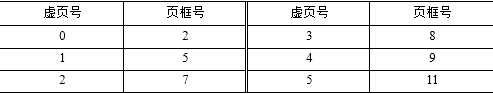
\includegraphics[width=3.33333in,height=0.63542in]{computerassets/b8801163b984bb0c1ef76b265a03fe84.jpeg}
\par\twoch{32773}{42773}{\textcolor{red}{12293}}{62773}
\begin{solution}C。 解法一:
对于本类题,先将物理地址转换为``物理页号+页内地址''的形式,然后查找页表以找出物理页号对应的逻辑页号,将``逻辑页号+页内地址''转换为对应的十进制数即可。
32773=32768+5=1000 0000 0000 0000B+101B=1000 0000 0000
0101B,后12位为页内地址,前4位为页号。物理页号为8,对应逻辑页号为3=11B。则逻辑地址=11
0000 0000 0101B= 3×4K+3=10240+2048+5=12288+5=12293。 解法二:
也可以不用化成二进制,直接通过除法得到的商和余数就可以得到答案。
32773÷4096(4K)=8余5,即其页框号为8,页内偏移量为5。查表,其对应的虚页号为3,则其虚拟地址=3×4096+5=12293。
\end{solution}
\question 某计算机采用二级页表的分页存储管理方式,按字节编制,页的大小为
\includegraphics[width=0.21875in,height=0.15625in]{texmath/e0c3285Cdpi7B3507D25E7B107D}字节,页表项大小为2字节,逻辑地址结构为:

~
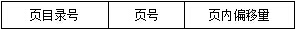
\includegraphics[width=3.08333in,height=0.31250in]{computerassets/caeb37c4933000ccb425f21fe0f14b7d.jpeg}~

逻辑地址空间大小为
\includegraphics[width=0.21875in,height=0.15625in]{texmath/0180d65Cdpi7B3507D25E7B167D}页,则表示整个逻辑地址空间的页目录表中包含表项的个数至少是(
~)
\par\twoch{64}{\textcolor{red}{128}}{256}{512}
\begin{solution}在内存中有些页是存储页表项的,相当于页的索引,本题就是要计算包含索引项的页的数量最小值是多少。由题可知每页的大小为
\includegraphics[width=0.21875in,height=0.15625in]{texmath/e0c3285Cdpi7B3507D25E7B107D}B,就是1024B,每个页表项的大小为2B,那么每页中可以存放512个页表项信息,逻辑地址总共有
\includegraphics[width=0.21875in,height=0.15625in]{texmath/0180d65Cdpi7B3507D25E7B167D}页,那么要储存全部2\^{}16个页表项所需要的页数量为
\includegraphics[width=0.21875in,height=0.15625in]{texmath/0180d65Cdpi7B3507D25E7B167D}/512=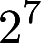
\includegraphics[width=0.15625in,height=0.15625in]{texmath/9558dc5Cdpi7B3507D25E7B77D}=128页,因此答案选B。
【总结】 ~ ~ ~
~有的书上也把这种存储方式叫做二级页表分页存储,将页号的前几位叫做页目录号,因此页表被分为了两级。
\end{solution}
